\documentclass[11pt, xcolor={dvipsnames}, hyperref={colorlinks, allcolors=Blue}]{beamer}


% Packages
\usepackage{graphicx}
\usepackage{caption, subcaption}
\usepackage{tikz}
\usepackage{amsmath, amsfonts, amssymb}
\usepackage{bm}
\usepackage{booktabs}
\usepackage{apacite}
\usepackage{multirow}
\usepackage{multicol}
\usepackage{doi}
\usepackage{textpos}
\usepackage{lipsum}
\usepackage{amsfonts, amsmath}
\usepackage{wrapfig}
\usepackage{animate}
\usepackage{cleveref}


\renewcommand\doiprefix{}


\usepackage{tikz}
\usetikzlibrary{shapes, fit}





%%%%%%%%%%%%%%%%%%%%%%%%%%%%%%%%%%%%%%%%%%%%%%
% Custom commands
\newcommand\bc[1]{{\usebeamercolor[fg]{frametitle} {\textbf{#1}}}} % bold and color
\newcommand{\into}{\rightarrow}



%%%%%%%%%%%%%%%%%%%%%%%%%%%%%%%%%%%%%%%%%%%%%%
% Set Theme
\usetheme{Boadilla}
\usecolortheme{rose}

%%%%%%%%%%%%%%%%%%%%%%%%%%%%%%%%%%%%%%%%%%%%%%
% Make citation font tiny
\renewcommand{\bibliographytypesize}{\tiny}

%%%%%%%%%%%%%%%%%%%%%%%%%%%%%%%%%%%%%%%%%%%%%%
% Fonts
\usefonttheme{serif} % Serif font
\setbeamertemplate{enumerate items}[default] % Don't use bullets in enumerate.

%%%%%%%%%%%%%%%%%%%%%%%%%%%%%%%%%%%%%%%%%%%%%%%
% Remove navigation bar
\setbeamertemplate{navigation symbols}{}
%%%%%%%%%%%%%%%%%%%%%%%%%%%%%%%%%%%%%%%%%%%%%%


% Frontmatter
\title[ECON 8000 -  Lecture 5]{Lecture 5: Probability}
\author[University of Queensland]{Robert Garrard}
\date[\today]{} 


%%%%%%%%%%%%%%%%%%%%%%%%%%%%%%%

% Common commands

% Sets
\newcommand{\R}{\mathbb{R}}
\newcommand{\N}{\mathbb{N}}
\newcommand{\Z}{\mathbb{Z}}
\newcommand{\Q}{\mathbb{Q}}
\renewcommand{\P}{\mathbb{P}}
\newcommand{\E}{\mathbb{E}}

% Symbols
\renewcommand{\epsilon}{\varepsilon}
\renewcommand{\implies}{\Rightarrow}
\newcommand{\halmos}{\hfill$\blacksquare$}

% Vector notation
\renewcommand{\a}{\mathbf{a}}
\renewcommand{\b}{\mathbf{b}}
\newcommand{\x}{\mathbf{x}}
\newcommand{\X}{\mathbf{X}}
\newcommand{\y}{\mathbf{y}}
\newcommand{\z}{\mathbf{z}}
\renewcommand{\v}{\mathbf{v}}
\newcommand{\bepsilon}{\mathbf{\varepsilon}}
\newcommand{\bbeta}{\mathbf{\beta}}

% Matrices
\newcommand{\eyetwo}{\begin{pmatrix} 1 & 0\\ 0 & 1 \\ \end{pmatrix}} % I_2 identity matrix
\newcommand{\eyethree}{\begin{pmatrix} 1 & 0 & 0\\ 0 & 1 & 0\\ 0 & 0 & 1 \end{pmatrix}} % I_3 identity matrix
\newcommand{\zerotwo}{\begin{pmatrix} 0 & 0\\ 0 & 0 \\ \end{pmatrix}} % 2x2 Zero matrix
\newcommand{\zerothree}{\begin{pmatrix} 0 & 0 & 0\\ 0 & 0 & 0\\ 0 & 0 & 0 \end{pmatrix}} % 3x3 Zero matrix


% Misc

\newcommand{\innerprod}[2]{\langle #1, #2 \rangle}


%%%%%%%%%%%%%%%%%%%%%%%%%%%%%%%%

% Tikz
\usetikzlibrary{arrows,shapes,trees, positioning}

%%%%%%%%%%%%%%%%%%%%%%%%%%%%%%

\newcounter{Lecture}
\addtocounter{Lecture}{5}

\newcounter{exercise}
\newenvironment{exercise}[1][]{\refstepcounter{exercise}\par\medskip
   \noindent {\bc{Exercise}~\bc{\theLecture.\theexercise} #1}}{\medskip}


\begin{document}

\begin{frame}
\titlepage

%\begin{picture}(0,0)
%\put(35,-50){\hbox{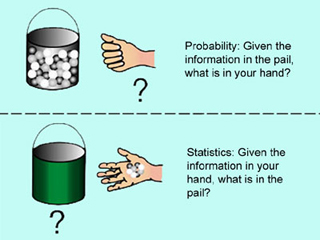
\includegraphics[width=0.8\textwidth, trim={0cm, 1cm, 0cm, 1cm}, clip]{prob_stats}}}
%\end{picture}

\end{frame}
%%%%%%%%%%%%%%%%%%%%%%%%%%%%%

\begin{frame}
\begin{figure}
	\centering
	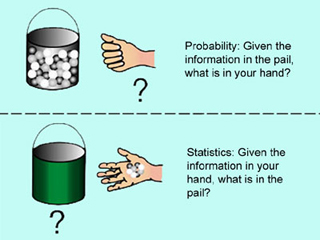
\includegraphics[width=0.66\textwidth]{prob_stats}
\end{figure}

\vfill
\textbf{Challange:} Without using the phrases ``chance'' or ``likelihood'', describe what a probability is.
\end{frame}
%%%%%%%%%%%%%%%%%%%%%%%%%%%%%

\begin{frame}{Axioms of Probability}
A \textbf{probability} is a function, $\P : 2^{\Omega} \to [0, 1]$ such that
\begin{enumerate}[1.]
\item $0 \leq \P(E) \leq 1$
\item $\P (\Omega) = 1$
\item For any countable sequence of \emph{disjoint} events $E_{i}$,
\[\P\left (\bigcup_{i=1}^{\infty} E_{i} \right) = \sum_{i=1}^{\infty} \P(E_{i}) \]
\end{enumerate}
\vfill

Probability \emph{measures} the size of sets in a particular way.

\vfill
\small
NB: This is not entirely correct. The domain of the function is not the whole power set but a subset that is a ``measurable space'' and $\P$ must be a ``measurable function'', but this is beyond our scope.
\end{frame}

%%%%%%%%%%%%%%%%%%%%%%%%%%%%%
\begin{frame}{Axioms of Probability}


\begin{exercise}
\begin{enumerate}
	\item Show that $\P (\emptyset) = 0$. 
	\item Show that $\P(E^{c}) = 1 - \P(E)$.
	\item Prove the inclusion-exclusion principle: $ \P(A \cup B) = \P(A) + \P(B) - \P(A \cap B)$
	\item Two fair coins are flipped. The person flipping the coins reveals to you that one of the coins is a head. Find the probability that the other is tails.


\end{enumerate}
\end{exercise}

\end{frame}

%%%%%%%%%%%%%%%%%%%%%%%%%%%%%
\begin{frame}{Conditional Probability}
Let $A$ and $B$ be events. The probability of $A$ \bc{conditional} on having observed $B$ is 
\[ \P(A|B) = \frac{\P(A \cap B)}{\P(B)}\]
\bigskip

Two events $A$ and $B$ are said to be \bc{independent} if 

\[\P(A \cap B) = \P(A)\cdot \P(B)\]

\vfill
\begin{exercise}

Apply this formula to the previous coin-flipping example.

\end{exercise}

\end{frame}

%%%%%%%%%%%%%%%%%%%%%%%%%%%%%

\begin{frame}{Law of Total Probability}
\begin{theorem}[Law of Total Probability]
Consider an event $A$. Let $B_{i}, \ \ i = 1,\dots,n$ be a partition of the sample space. That is, $B_{i} \cap B_{j} = \emptyset \ \ \forall i,j$ and $\bigcup_{i=1}^{n} B_{i} = \Omega$.

\[ \P(A) = \sum_{i=1}^{n} \P(A \cap B_{i})\]
\end{theorem}

It's often useful to substitute the conditional probability formula to make the theorem

\[\P(A) = \sum_{i=1}^{n} \P(A|B_{i}) \P(B_{i})\]

\end{frame}
%%%%%%%%%%%%%%%%%%%%%%%%%%%%%
\begin{frame}{Law of Total Probability}
\begin{exercise}


Consider two urns. The first contains two white and seven black balls, and the second contains five white and six black balls. We flip a fair coin and then
draw a ball from the first urn or the second urn depending on whether the outcome was heads or tails.\bigskip

What is the probability of drawing a white ball? 
\end{exercise}
\end{frame}

%%%%%%%%%%%%%%%%%%%%%%%%%%%%%
\begin{frame}{Bayes' Theorem}
Bayes' theorem gives us a way to invert conditional probabilities. 

\begin{theorem}{Bayes' Theorem}
Let $A$ and $B$ be events such that $\P(B) > 0$.

\[ \P(A | B) = \frac{\P(B | A) \P(A)}{\P(B)}\]

\end{theorem}
\bigskip 

Bayes' theorem is often more easily applied by substituting the law of total probability into the denominator

\[ \P(A_{i}|B) = \frac{\P(B|A_{i}) \P(A_{i})}{\sum_{i} \P(B|A_{i}) \P(A_{i})}\]

\end{frame}

%%%%%%%%%%%%%%%%%%%%%%%%%%%%%
\begin{frame}{Bayes' Theorem}

\begin{exercise}
A blood test is 95 percent effective in detecting a certain disease when it is, in fact, present. However, the test also yields a “false positive” result for 1 percent of the healthy persons tested. If 0.5 percent of the population actually has the disease, what is the probability a person has the disease given that his test result is positive?


\end{exercise}
\vfill\vfill

\end{frame}
%%%%%%%%%%%%%%%%%%%%%%%%%%%%%
\begin{frame}{Random Variables}

It frequently occurs that in performing an experiment we are mainly interested in some
functions of the outcome as opposed to the outcome itself.\bigskip

These quantities of interest, or more formally, these real-valued
functions defined on the sample space, are known as \bc{random variables}.\bigskip

\begin{block}{Dice Rolling}
Let $X:\Omega \to \R$,  be the random variable defined by the sum of two fair dice.
\begin{align*}
&\P(X = 2) = \P\{(2,2)\} = 1/36\\
&\P(X = 3) = \P\{(1,2), (2,1)\} = 2/36\\
&\P(X = 4) = \P\{(1,3), (2,2), (3,1)\} = 3/36\\
&\text{etc}
\end{align*}
\end{block}
\end{frame}


%%%%%%%%%%%%%%%%%%%%%%%%%%%%%
\begin{frame}{Random Variables}

The \bc{cumulative distribution function} (cdf), $F(\cdot)$, of the random variable X is defined for any real number $b \in \R$, by
\[F(b) = \P(X \leq b)\]

Some properties of the cdf $F$ are:

\begin{enumerate}[i)]
\item $F(b)$ is a nondecreasing function of $b$
\item $\lim_{b\to\infty} F(b) = F(\infty) = 1$
\item $\lim_{b\to - \infty} F(b) = F(-\infty) = 0$
\end{enumerate}
\bigskip

All probability questions about X can be answered in terms of the cdf $F(\cdot)$.



\end{frame}
%%%%%%%%%%%%%%%%%%%%%%%%%%%%%
\begin{frame}{Discrete Random Variables}
When the image of a random variable, $X:\Omega \to \R$, is countable, we say that it is a \bc{discrete} random variable.\bigskip

For discrete rvs, we define the \bc{probability mass function} (pmf) to be:
\[p_{X}(x_{i}) = \P(X = x_{i})\]
\bigskip

This has the usual properties: $\forall x_{i} \ p_{X}(x_{i}) \geq 0$, and $\sum_{i} p_{X}(x_{i}) = 1$.\bigskip

The pmf and cdf are related by:

\begin{center}
\begin{tabular}{cc}
$p_{X}(x_{i}) = F(x_{i}) - F(x_{i-1})$ &\quad $F(x_{i}) = \sum_{j \leq i } p_{X}(x_{j})$
\end{tabular}
\end{center}
\end{frame}

%%%%%%%%%%%%%%%%%%%%%%%%%%%%%
\begin{frame}{Common Discrete Random Variables}

\begin{figure}[t]
	\begin{subfigure}[b]{0.4\textwidth}
		\centering
		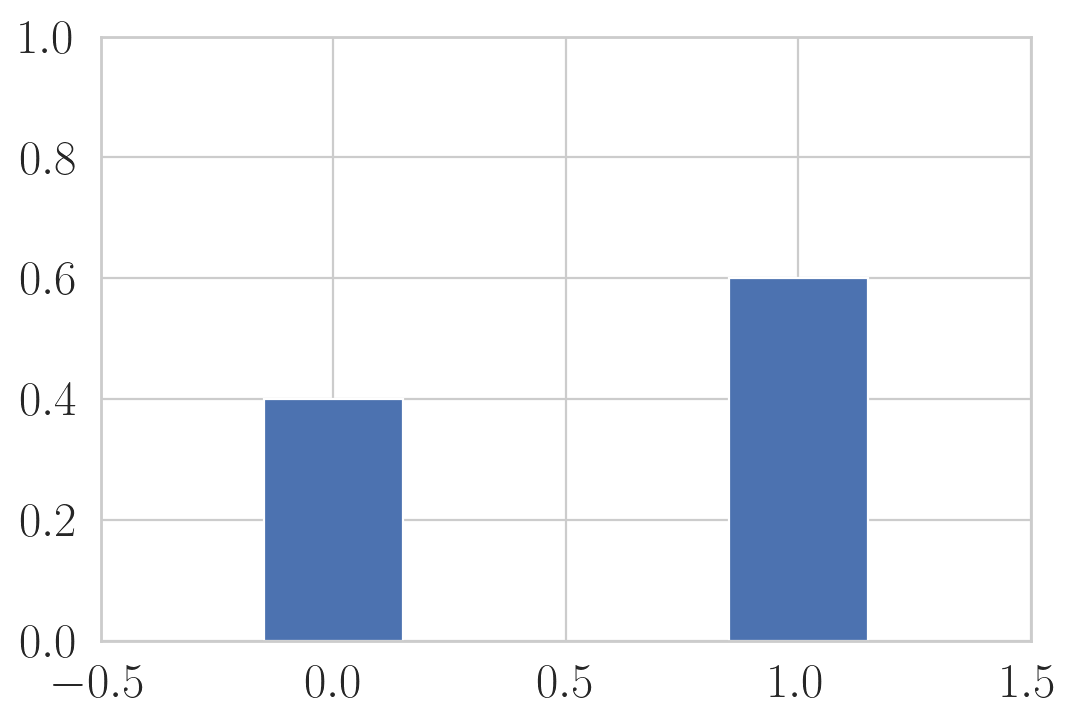
\includegraphics[width=\textwidth]{bernoulli_pmf.png}
		\caption*{PMF}
	\end{subfigure}
	\begin{subfigure}[b]{0.4\textwidth}
		\centering
		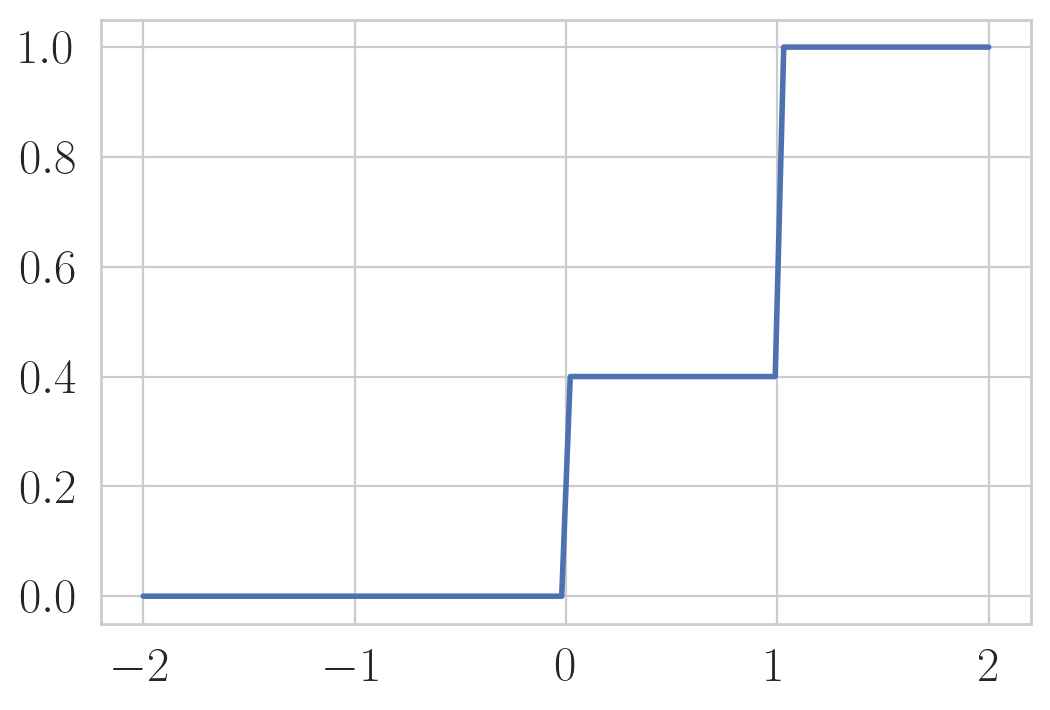
\includegraphics[width=\textwidth]{bernoulli_cdf.png}
		\caption*{CDF}
	\end{subfigure}
\caption{Bernoulli random variable}
\end{figure}

\begin{center}
\begin{tabular}{cc}
$f(k; p) = \begin{cases} p & \text{if } k=1 \\ 1-p & \text{if } k = 0\end{cases}$ & \ 
$F(x; p) = \begin{cases} 0 & \text{if } x< 0 \\ 1-p & \text{if } 0 \leq x < 1 \\1 & \text{if } x \geq 1  \end{cases}$
\end{tabular}
\end{center}

\end{frame}

%%%%%%%%%%%%%%%%%%%%%%%%%%%%%
\begin{frame}{Common Discrete Random Variables}

\begin{figure}[t]
	\begin{subfigure}[b]{0.4\textwidth}
		\centering
		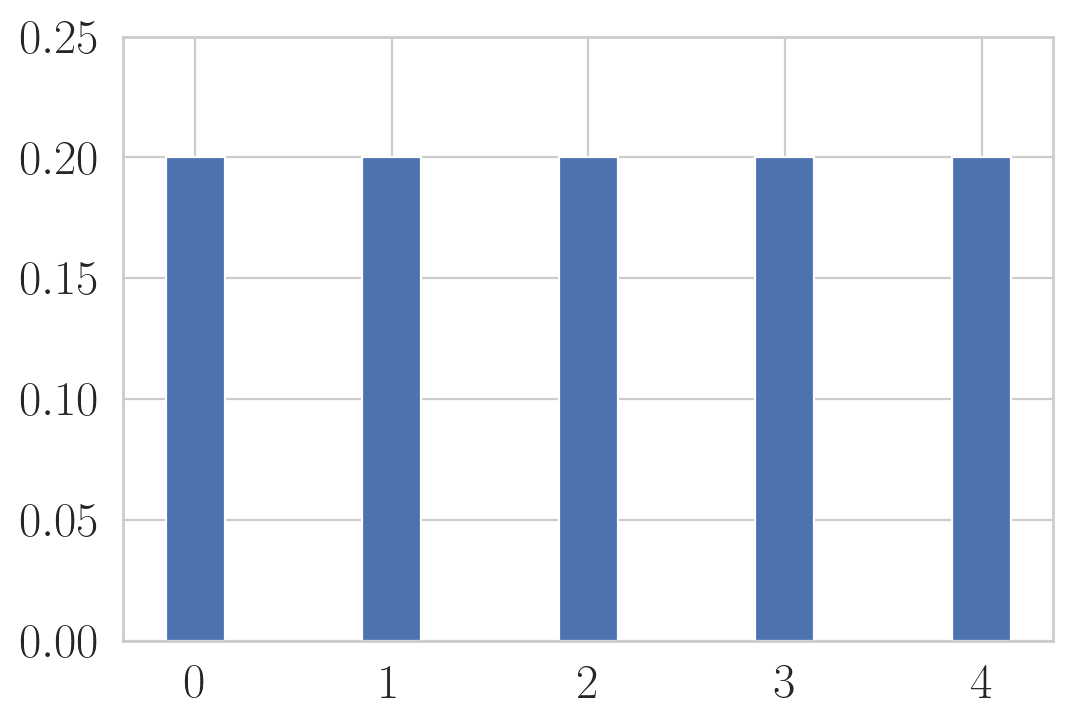
\includegraphics[width=\textwidth]{discrete_uniform_pmf.png}
		\caption*{PMF}
	\end{subfigure}
	\begin{subfigure}[b]{0.4\textwidth}
		\centering
		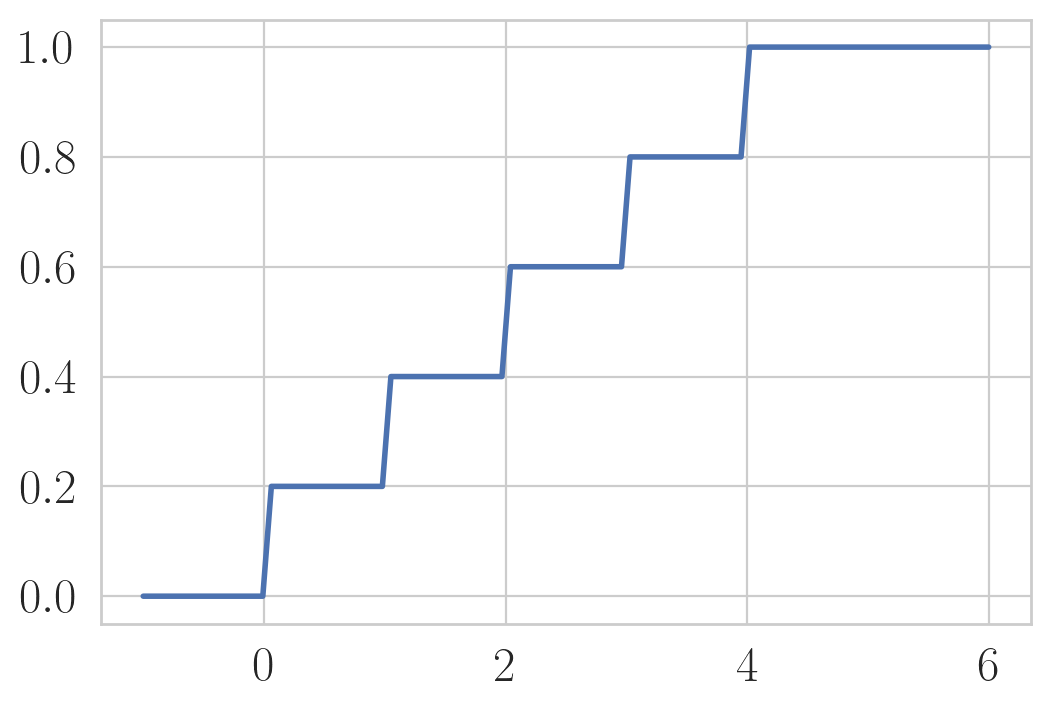
\includegraphics[width=\textwidth]{discrete_uniform_cdf.png}
		\caption*{CDF}
	\end{subfigure}
\caption{Discrete Uniform}
\end{figure}

\begin{center}
\begin{tabular}{cc}
$f(k; a, b) = \begin{cases} \frac{1}{b-a+1} & \text{if } k\in\{a, a+1, \dots, b\} \\ 0 & \text{Otherwise} \end{cases}$ & \ 
$F(x; a, b) = \frac{\lfloor k \rfloor - a + 1}{b-a+1}$
\end{tabular}
\end{center}

\end{frame}

%%%%%%%%%%%%%%%%%%%%%%%%%%%%%
\begin{frame}{Common Discrete Random Variables}

\begin{figure}[t]
	\begin{subfigure}[b]{0.4\textwidth}
		\centering
		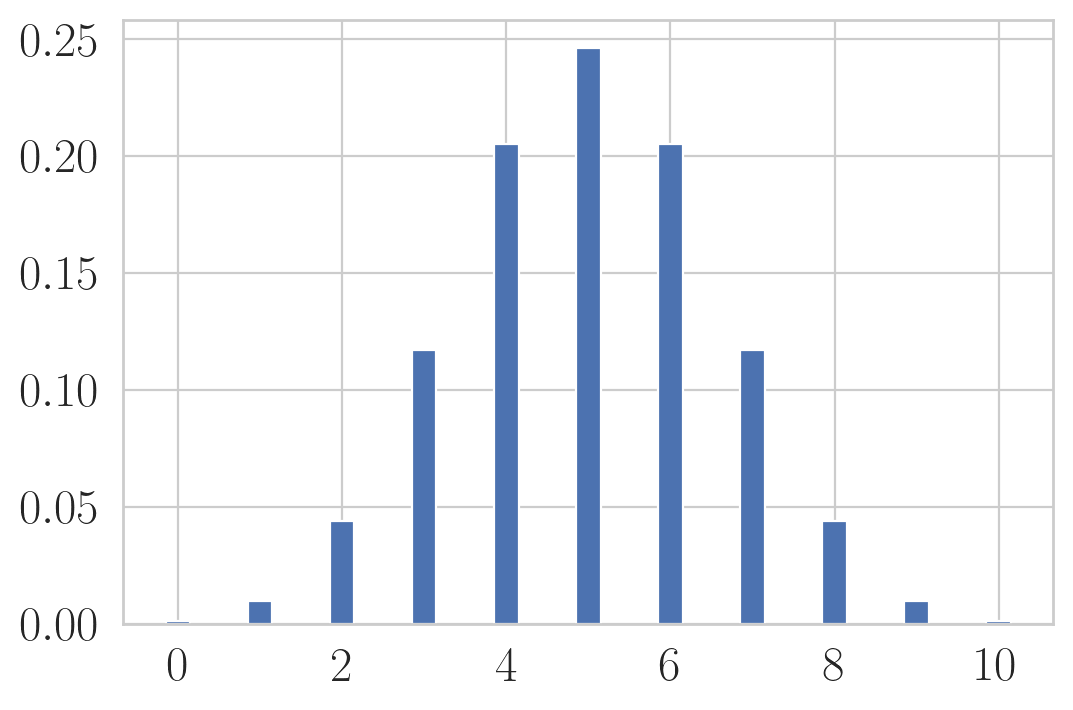
\includegraphics[width=\textwidth]{binomial_pmf.png}
		\caption*{PMF}
	\end{subfigure}
	\begin{subfigure}[b]{0.4\textwidth}
		\centering
		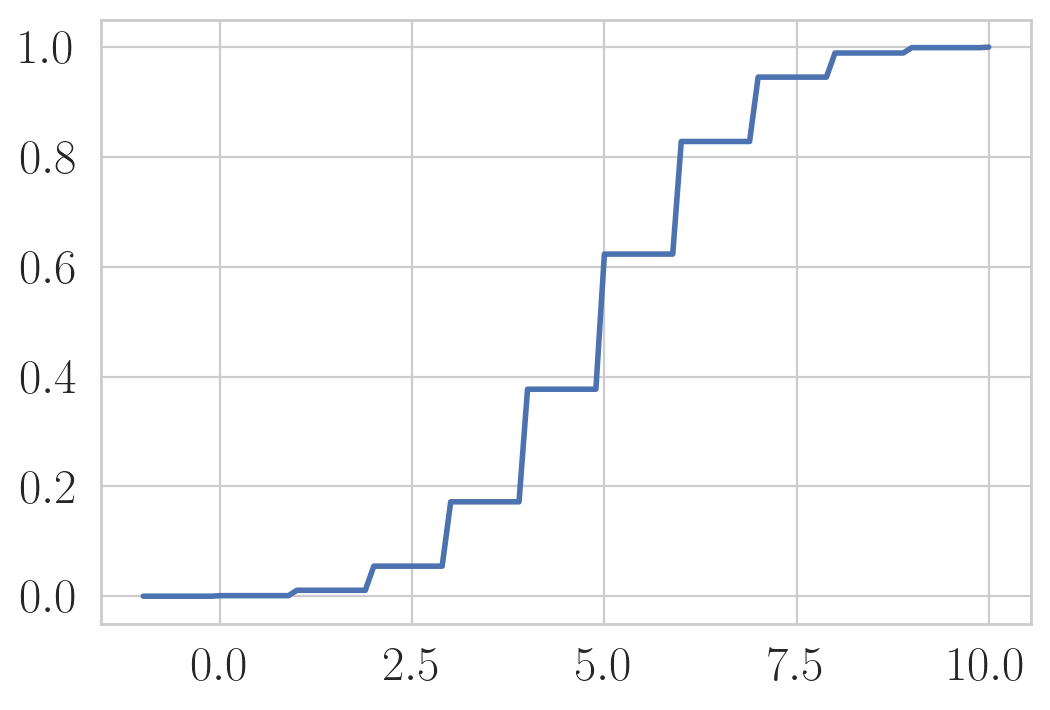
\includegraphics[width=\textwidth]{binomial_cdf.png}
		\caption*{CDF}
	\end{subfigure}
\caption{Binomial}
\end{figure}


\[f(k; n, p) = \binom{n}{k} p^{k} (1-p)^{n-k}\]

\end{frame}
%%%%%%%%%%%%%%%%%%%%%%%%%%%%%
\begin{frame}{Common Discrete Random Variables}

\begin{figure}[t]
	\begin{subfigure}[b]{0.4\textwidth}
		\centering
		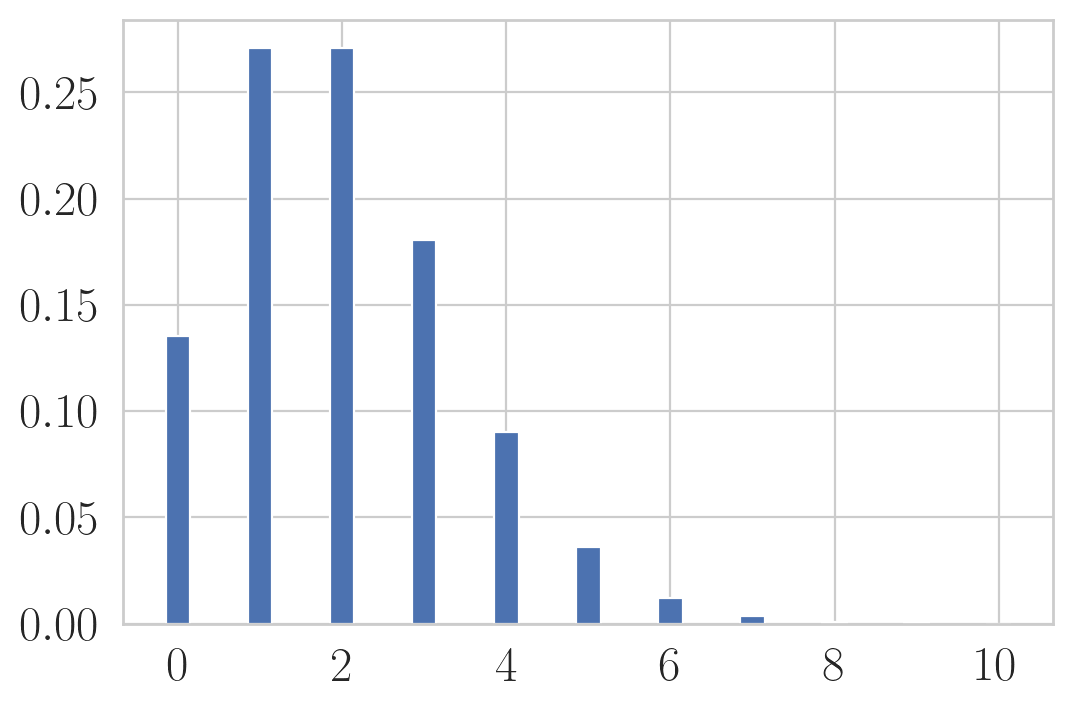
\includegraphics[width=\textwidth]{poisson_pmf.png}
		\caption*{PMF}
	\end{subfigure}
	\begin{subfigure}[b]{0.4\textwidth}
		\centering
		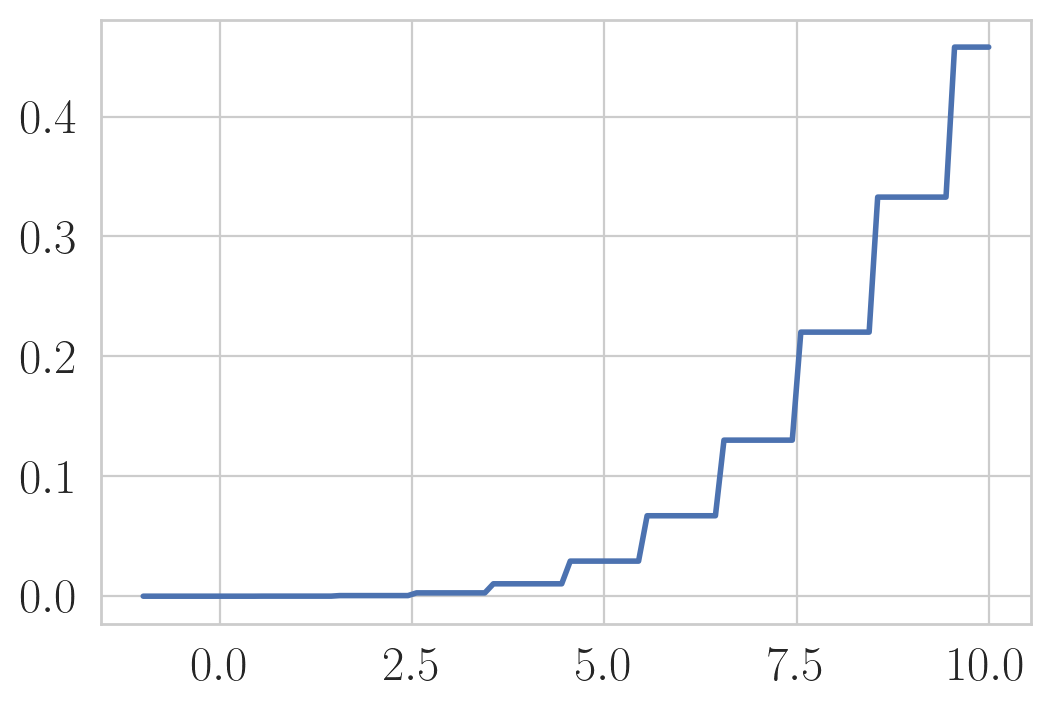
\includegraphics[width=\textwidth]{poisson_cdf.png}
		\caption*{CDF}
	\end{subfigure}
\caption{Poisson}
\end{figure}


\[f(k; \lambda) = \frac{\lambda^{k} e^{-\lambda}}{k!}\]
\end{frame}

%%%%%%%%%%%%%%%%%%%%%%%%%%%%%
\begin{frame}{Common Discrete Random Variables}

\begin{exercise}


Show that the poisson pmf is a valid pmf.
\end{exercise}

\vfill\vfill\vfill
\end{frame}

%%%%%%%%%%%%%%%%%%%%%%%%%%%%%

\begin{frame}{Continuous Random Variables}

When the cdf of a random variable is continuous everywhere, we call it a \bc{continuous} random variable.\bigskip

If the cdf is \bc{absolutely continuous} it admits a \bc{probability density function} (pdf), $f(x)$, where: 

\[\forall x \ f(x) \geq 0 \qquad \int_{\infty}^{\infty} f(x) \mathrm{d}x = 1\]

\[F(b) = \int_{-\infty}^{b} f(x) \mathrm{d}x\]
\[\P(a \leq X \leq b) = \int_{a}^{b} f(x) \mathrm{d}x\]

\[\frac{\mathrm{d}}{\mathrm{d}x} F(x) = f(x)\]
\end{frame}
%%%%%%%%%%%%%%%%%%%%%%%%%%%%%

\begin{frame}{Common Continuous Random Variables}

\begin{figure}[t]
	\begin{subfigure}[b]{0.4\textwidth}
		\centering
		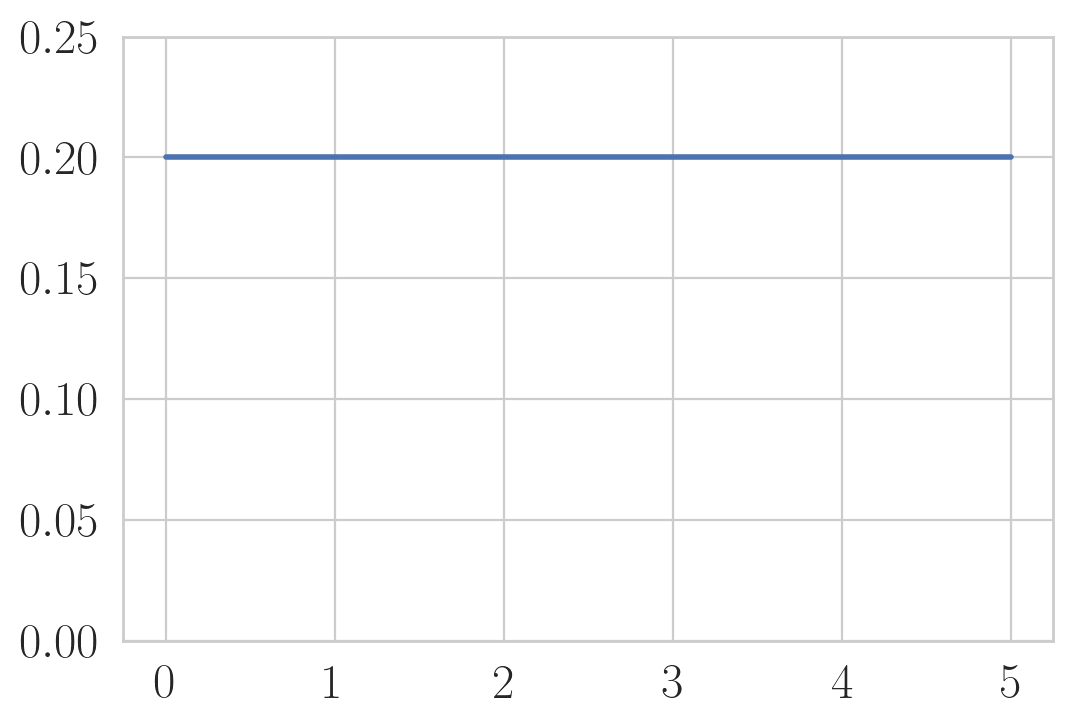
\includegraphics[width=\textwidth]{continuous_uniform_pdf.png}
		\caption*{PDF}
	\end{subfigure}
	\begin{subfigure}[b]{0.4\textwidth}
		\centering
		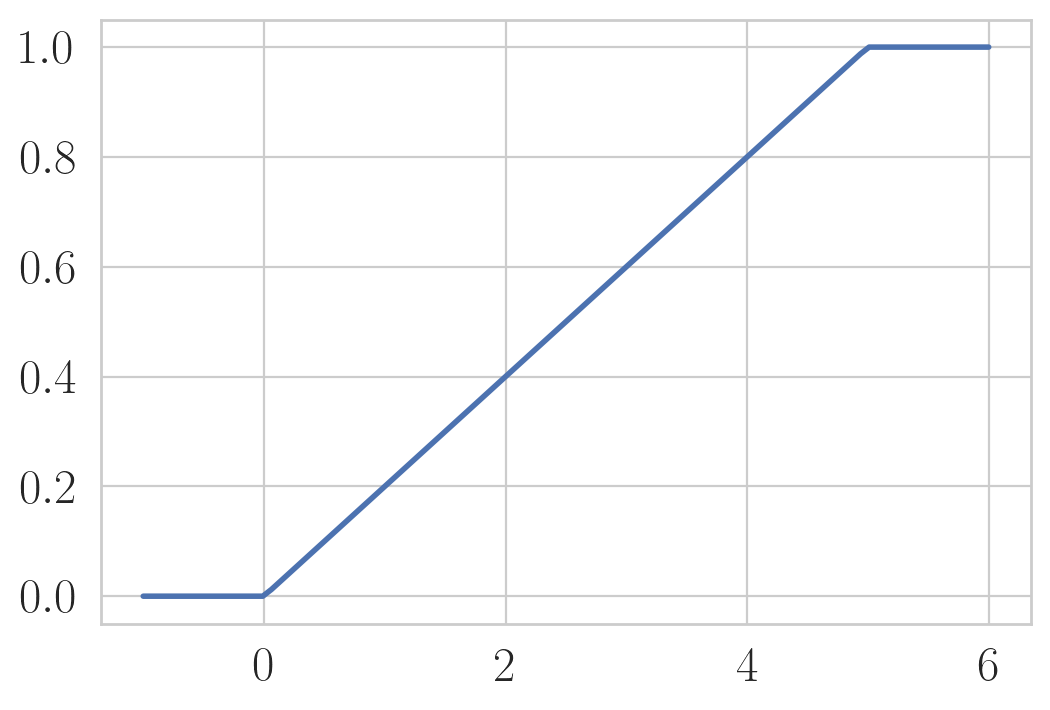
\includegraphics[width=\textwidth]{continuous_uniform_cdf.png}
		\caption*{CDF}
	\end{subfigure}
\caption{Discrete Uniform}
\end{figure}

\begin{center}
\begin{tabular}{cc}
$f(x; a, b) = \begin{cases}\frac{1}{b-a} \quad \text{if} \ x \in (a,b)\\0 \quad \text{otherwise}\end{cases}$ & \ 
$F(x; a, b) = \begin{cases} 0 & x < a \\ \frac{x-a}{b-a} & x \in [a, b] \\ 1 & x> b\end{cases}$
\end{tabular}
\end{center}



\end{frame}
%%%%%%%%%%%%%%%%%%%%%%%%%%%%%

\begin{frame}{Common Continuous Random Variables}
\begin{figure}[t]
	\begin{subfigure}[b]{0.4\textwidth}
		\centering
		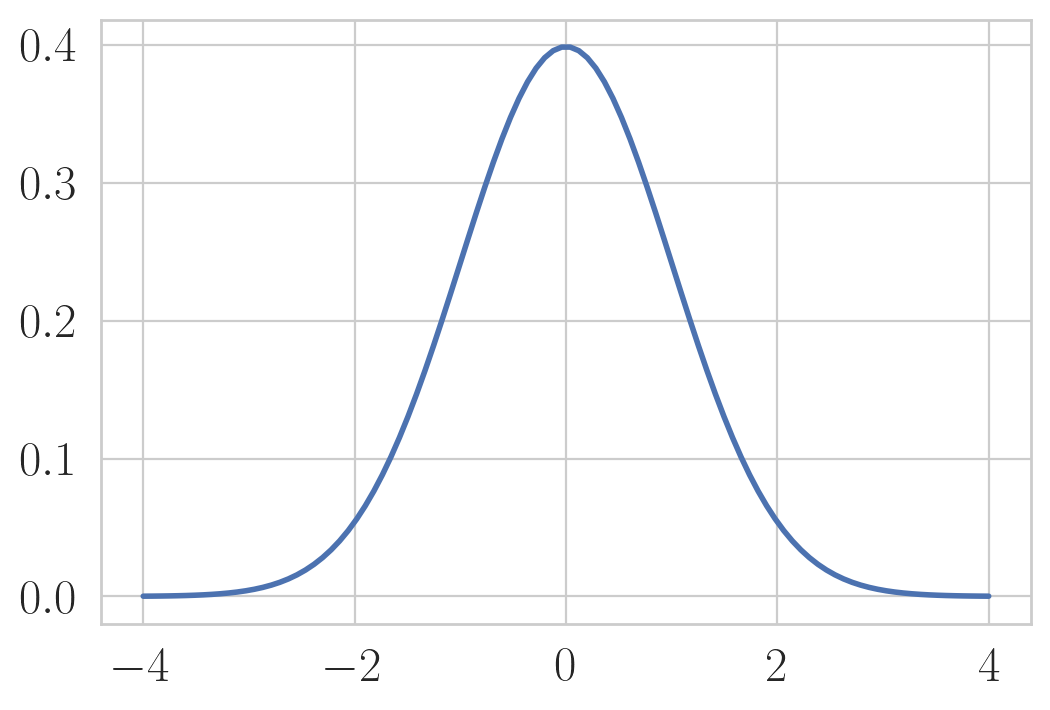
\includegraphics[width=\textwidth]{normal_pdf.png}
		\caption*{PDF}
	\end{subfigure}
	\begin{subfigure}[b]{0.4\textwidth}
		\centering
		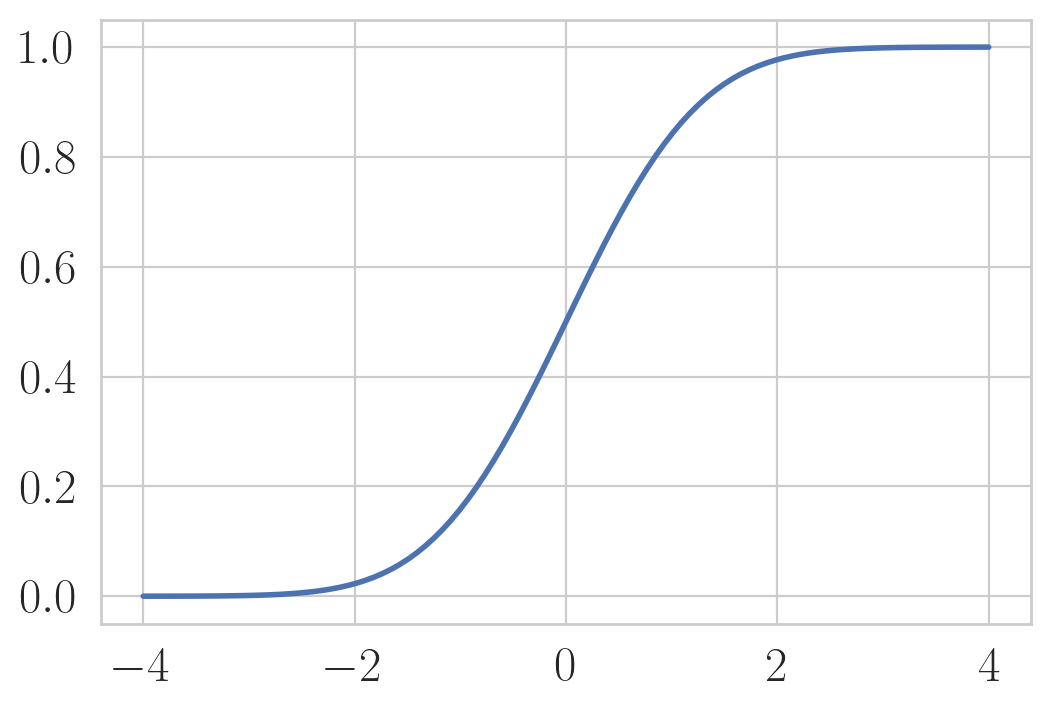
\includegraphics[width=\textwidth]{normal_cdf.png}
		\caption*{CDF}
	\end{subfigure}
\caption{Normal}
\end{figure}

\[ f(x; \mu, \sigma^{2}) = \frac{1}{\sigma^{2}\sqrt{2\pi}} e^{-\frac{1}{2} \left(\frac{x - \mu}{\sigma}\right)^{2}} \quad \ -\infty < x < \infty \]


\end{frame}

%%%%%%%%%%%%%%%%%%%%%%%%%%%%%

\begin{frame}{Common Continuous Random Variables}
\begin{figure}[t]
	\begin{subfigure}[b]{0.4\textwidth}
		\centering
		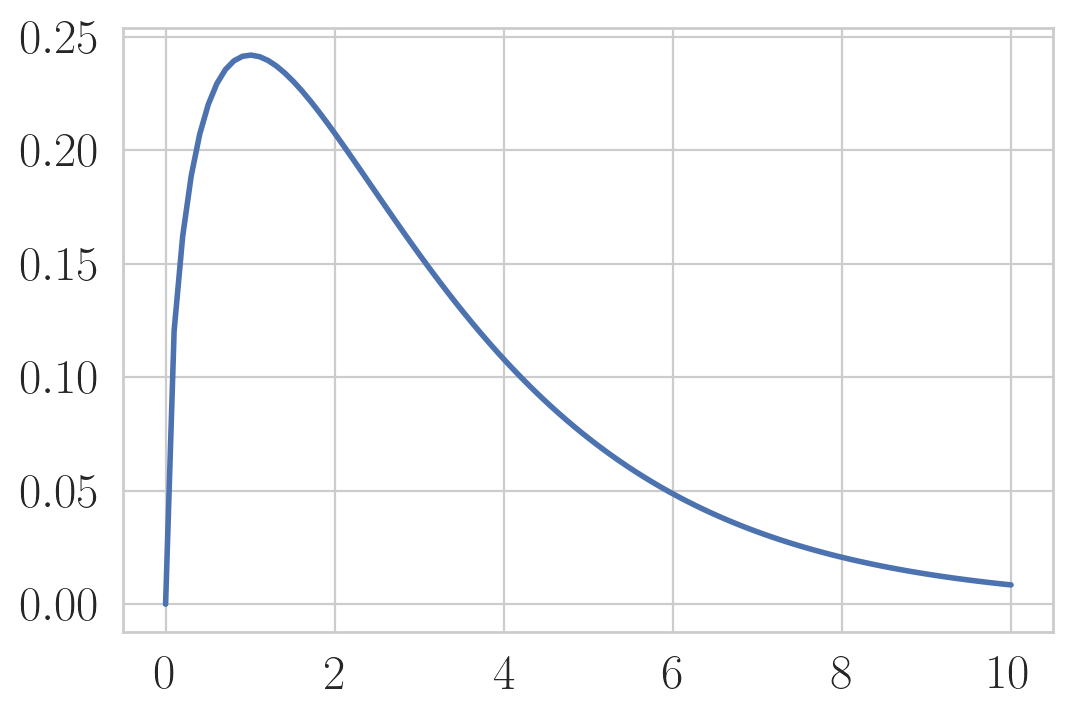
\includegraphics[width=\textwidth]{chisquare_pdf.png}
		\caption*{PDF}
	\end{subfigure}
	\begin{subfigure}[b]{0.4\textwidth}
		\centering
		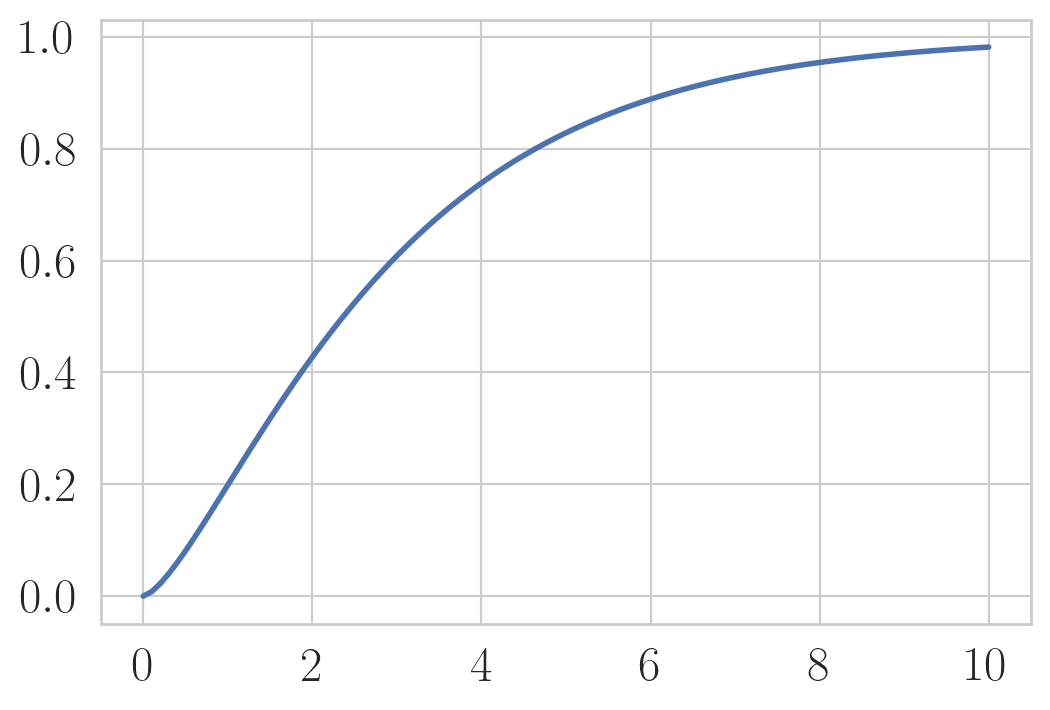
\includegraphics[width=\textwidth]{chisquare_cdf.png}
		\caption*{CDF}
	\end{subfigure}
\caption{Chi-square}
\end{figure}


Let $Z_1,\dots,Z_v$ be  $v$ independent standard normal distributions.

\[ \sum_{i=1}^{v}Z^{2}_i \sim \chi^{2}(v)\] 

\end{frame}

%%%%%%%%%%%%%%%%%%%%%%%%%%%%%

\begin{frame}{Common Continuous Random Variables}

\begin{figure}[t]
	\begin{subfigure}[b]{0.4\textwidth}
		\centering
		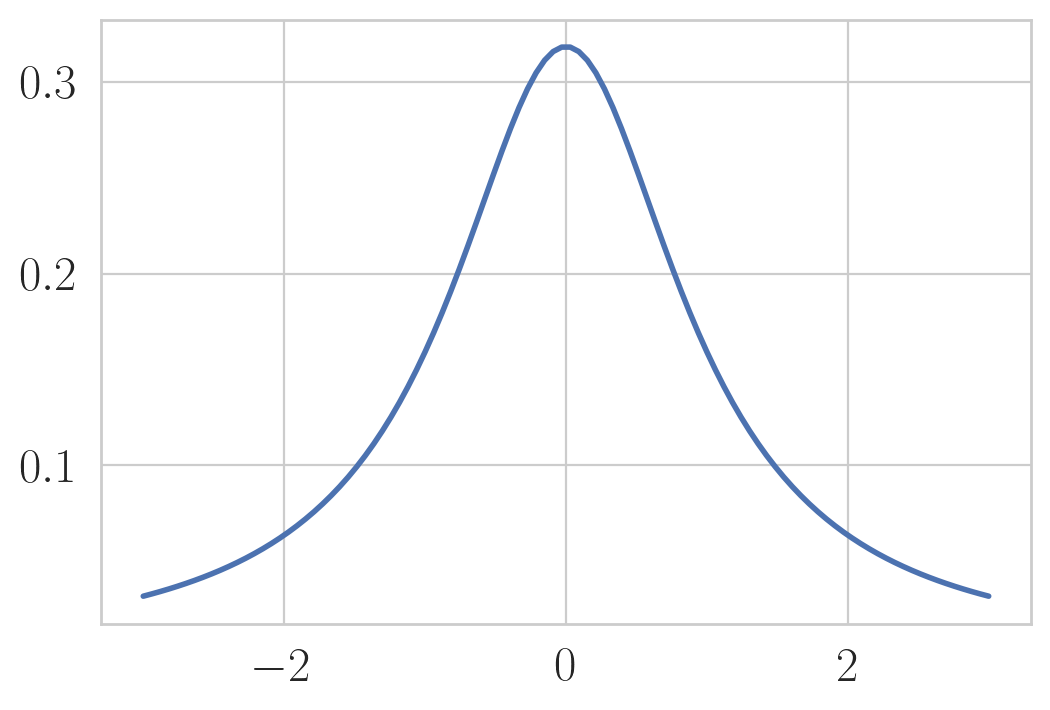
\includegraphics[width=\textwidth]{t_pdf.png}
		\caption*{PDF}
	\end{subfigure}
	\begin{subfigure}[b]{0.4\textwidth}
		\centering
		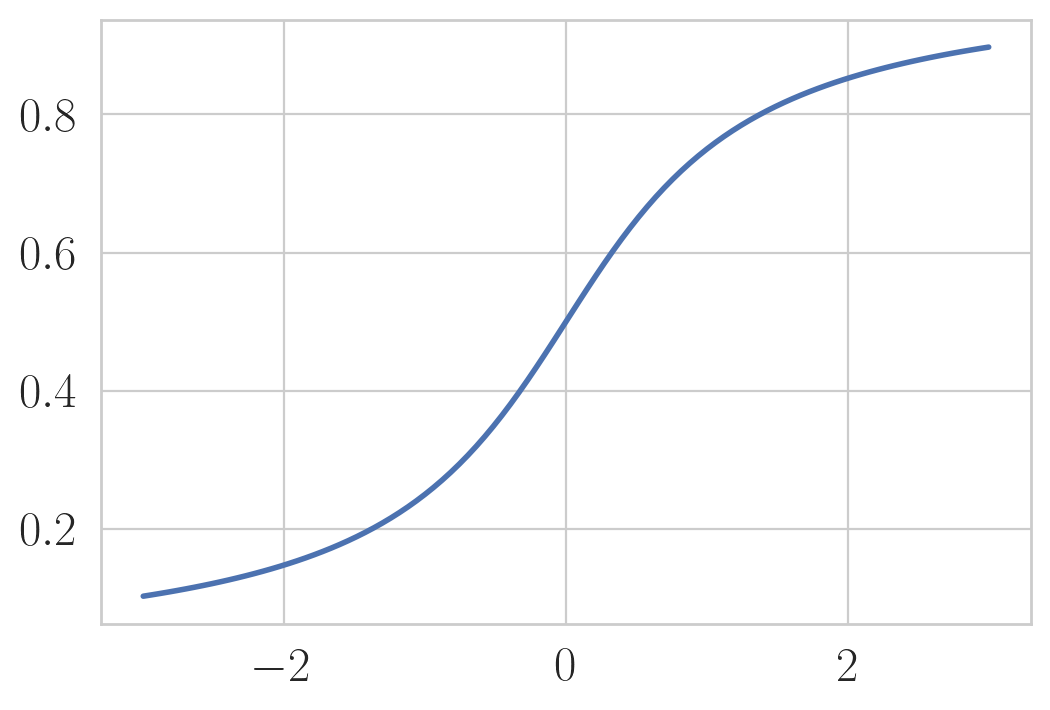
\includegraphics[width=\textwidth]{t_cdf.png}
		\caption*{CDF}
	\end{subfigure}
\caption{Student's $t$}
\end{figure}



Let $Z \sim N(0,1)$ and $V \sim \chi^{2}(v)$ , $Z$ and $V$ independent.	

\[ \frac{Z}{\sqrt{V/v}} \sim t(v)\]

\end{frame}
%%%%%%%%%%%%%%%%%%%%%%%%%%%%%

\begin{frame}{Common Continuous Random Variables}
\begin{figure}[t]
	\begin{subfigure}[b]{0.4\textwidth}
		\centering
		\includegraphics[width=\textwidth]{f_pdf.png}
		\caption*{PDF}
	\end{subfigure}
	\begin{subfigure}[b]{0.4\textwidth}
		\centering
		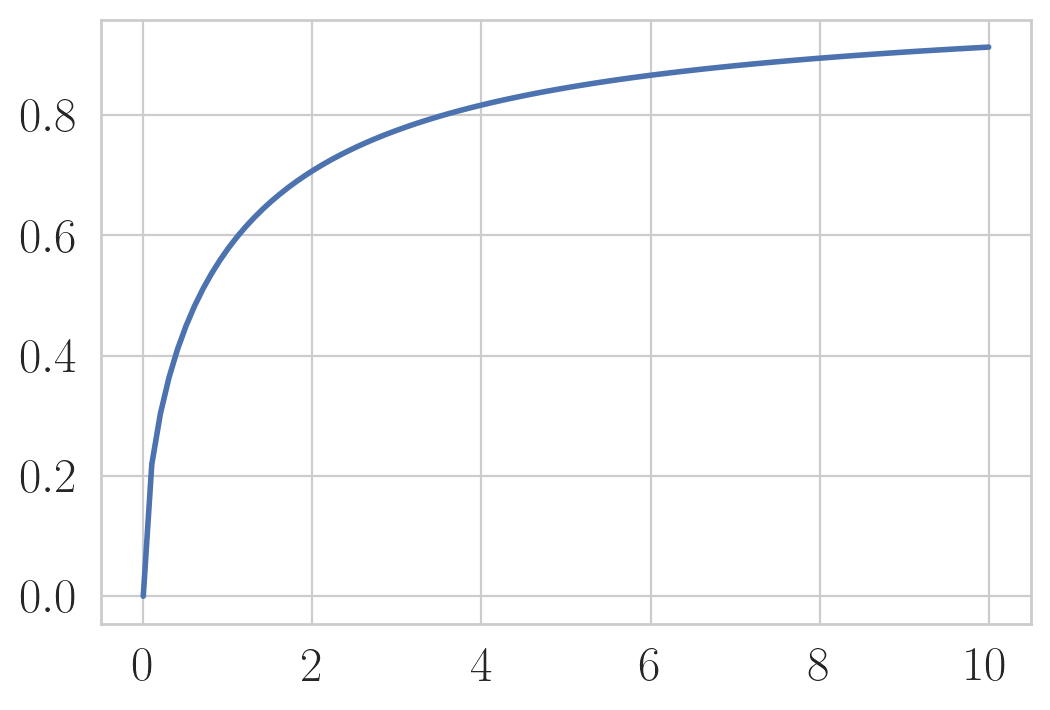
\includegraphics[width=\textwidth]{f_cdf.png}
		\caption*{CDF}
	\end{subfigure}
\caption{Fisher}
\end{figure}


Let $X \sim \chi^2(d_1)$ and $Y \sim \chi^2(d_2)$. 

\[ \frac{X/d_1}{Y/d_2} \sim F(d_1, d_2)\]


\end{frame}

%%%%%%%%%%%%%%%%%%%%%%%%%%%%%

\begin{frame}{Expectation}
\bc{Discrete Case:}\\

If X is a discrete random variable having a probability mass function $\P(x)$, then the expected value of X is defined by

\[ \E[X] = \sum_{x} x\cdot \P(x) \]

\bc{Continuous Case:}\\

If X is a continuous random variable having a probability density function $f (x)$, then the expected value of X is defined by

\[ \E[X] = \int_{-\infty}^{\infty} x f(x) \mathrm{d}x \]

\vfill
For this to be well defined, we require that $\E[|X|] < \infty$.
\end{frame}
%%%%%%%%%%%%%%%%%%%%%%%%%%%%%

\begin{frame}{Expectation}

\begin{theorem}
\begin{enumerate}[(a)]
\item If X is a discrete random variable with probability mass function $\P(x)$, then for any real-valued function $g$,
\[ \E[g(X)] = \sum_{x} g(x) \P(x) \]

\item  If X is a continuous random variable with probability density function $f(x)$, then for any real-valued function $g$,
\[ \E[g(X)] = \int_{-\infty}^{\infty} g(x)f(x) \mathrm{d}x\]
\end{enumerate}
\end{theorem}
\end{frame}

%%%%%%%%%%%%%%%%%%%%%%%%%%%%%

\begin{frame}{Expectation}

\begin{exercise}
\begin{enumerate}
	\item Show that if $a$ and $b$ are constants, $\E[ aX + b] = a \E[X] + b$.
	\item I throw a dart uniformly at random at a dart board of unit radius. On average, what will be the distance my dart lands from the bullseye?
\end{enumerate}
\end{exercise}

\vfill\vfill

\end{frame}

%%%%%%%%%%%%%%%%%%%%%%%%%%%%%

\begin{frame}{Economic Application: Decision Under Uncertainty}

A simple \bc{lottery} is a list $L = \{p_{1}, \dots, p_{N}\}$, with $p_{n} \geq 0$, $\sum_{n} p_{n} = 1$, where $p_{n}$ is the interpreted as the probability of outcome $n$ occurring.\bigskip

We can form \bc{compound lotteries}, $(L_{1}, \dots, L_{k}; \alpha_{1}, \dots, \alpha_{k})$, that yields the simple lottery $L_{i}$ with probability $\alpha_{i}$.\bigskip

Define a preference relation on the space of lotteries to be \bc{continuous} if for any $L, L^{\prime}, L^{\prime\prime}$, the sets
\[\{\alpha \in [0, 1] : \alpha L + (1-\alpha) L^{\prime} \succsim L^{\prime\prime}\}\]
\[\{\alpha \in [0, 1] : \alpha L + (1-\alpha) L^{\prime} \precsim L^{\prime\prime}\}\]

are closed.
\end{frame}


\begin{frame}{Economic Application: Decision Under Uncertainty}
The preference relation satisfies the \bc{independence axiom} if for all $L, L^{\prime}, L^{\prime\prime}$ 

\[L \succsim L^{\prime} \iff \alpha L + (1- \alpha) L^{\prime} \succsim \alpha L^{\prime} + (1-\alpha) L^{\prime\prime}\]

\begin{theorem}{Expected Utility Theorem}
Suppose a rational preference relation, $\succeq$, on the set of lotteries satisfies the continuity and independence axioms. Then $\succeq$ can be represented in expected utility form
\[L \succeq L^{\prime} \iff \E_{L}[U] \geq \E_{L^{\prime}}[U]\]

for some utility function $U$.
\end{theorem}
\end{frame}
%%%%%%%%%%%%%%%%%%%%%%%%%%%%%
\begin{frame}{Variance}

The \bc{variance} of a random variable X is defined as

\[ \mathrm{Var}(X) = \E \left [  (X - \E[X])^{2}   \right] \]

often written more compactly as

\[\mathrm{Var}(X) = \E [X^{2}] - \E[X]^{2}\]

\vfill
\begin{exercise}
\begin{enumerate}
	\item Show that $\mathrm{Var}(aX + b) = a^{2}\mathrm{Var}(X)$.
\end{enumerate}
\end{exercise}
\end{frame}

%%%%%%%%%%%%%%%%%%%%%%%%%%%%%
\begin{frame}{Moments}

The $k$-th \bc{central moment} is defined as 

\[\mu_{k} = \E[(X - \E[X])^{k}]\]\bigskip

The $k$-th \bc{raw moment} is defined as 

\[\mu_{k}^{\prime} = \E[X^{k}]\]\bigskip

If the $n$th moment exists, so does the $(n-1)$th.

\end{frame}
%%%%%%%%%%%%%%%%%%%%%%%%%%%%%
\begin{frame}{Moment Generating Functions}

If all of the moments exist, we can talk about the \bc{moment generating function}.

\[M_{X}(t) = \E[e^{tX}]\]

\bigskip

The MGF has the following useful properties:
\begin{enumerate}
	\item If random variables $X$ and $Y$ have the same MGF, they have the same distribution.
	\item If $X$ and $Y$ are independent random variables, then their sum $X + Y$ has MGF: $M_{X+Y}(t) = M_{X}(t) \cdot M_{Y}(t)$.
	\item $M_{cX}(t) = M_{X}(ct)$.
	\item $\mu_{k}^{\prime} = \left. \frac{\mathrm{d}^{n}M_{X}}{\mathrm{d}t^{n}}\right\vert_{t=0}$
\end{enumerate}
\end{frame}

%%%%%%%%%%%%%%%%%%%%%%%%%%%%%
\begin{frame}{Moment Generating Functions}

\begin{exercise}
\begin{enumerate}
	\item Show that the standard normal distribution has MGF: $M_{Z}(t) = e^{\frac{1}{2}t^{2}}$.
	\item Let $X\sim N(\mu, \sigma^{2})$. This has MGF $M_{X}(t) = e^{\mu t + \sigma^{2} t^{2} / 2}$.\bigskip

 Show that if $X_{1} \sim N(\mu_{1}, \sigma^{2}_{1})$ and $X_{2} \sim N(\mu_{2}, \sigma^{2}_{2})$ are independent random variables, then if $Y = X_{1} + X_{2}$ is the sum, $Y \sim N(\mu_{1} + \mu_{2}, \sigma^{2}_{1} + \sigma^{2}_{2})$.

	\item Show that if $X \sim N(\mu, \sigma^{2})$, then $aX \sim N(a\mu, a^{2}\sigma^{2})$.
\end{enumerate}
\end{exercise}

\end{frame}

%%%%%%%%%%%%%%%%%%%%%%%%%%%%%
\begin{frame}{Jointly Distributed Random Variables}

Thus far we've concerned ourselves only with the probability distribution of a single random variable.

\bigskip

 However, we are often interested in probability statements concerning two or more random variables. \bigskip

To deal with such probabilities, we define, for any two random variables X and Y, the \bc{joint cumulative distribution function} of X and Y by

\[ F(a,b) = \P(X \leq a, Y \leq b) \quad \ -\infty < a,b < \infty\]

\end{frame}
%%%%%%%%%%%%%%%%%%%%%%%%%%%%%
\begin{frame}{Jointly Distributed Random Variables}

The \bc{marginal} distribution of X can be obtained from the joint distribution as follows

\begin{align*}
F_{X}(a) &= \P(X \leq a)\\
&= \P(X \leq a, Y \leq \infty)\\
&= F(a, \infty)
\end{align*}

Similarly for the CDF of Y.\\

As before, we'll talk about the \bc{joint pmf} or \bc{joint density}, $\P(x,y) = \P(X = x, Y = y)$. From this the marginal distributions are

\[\P_{X}(x) = \sum_{y} \P(x,y) \qquad \P_{X}(x) = \int_{-\infty}^{\infty}\P(x,y) \mathrm{d}y\]

\end{frame}

%%%%%%%%%%%%%%%%%%%%%%%%%%%%%
\begin{frame}{Covariance}

The \bc{covariance} of any two random variables, X and Y, is

\[ \mathrm{Cov}(X,Y) = \E[(X - \E[X])(Y - \E[Y])]\]

or sometimes more conveniently

\[\mathrm{Cov}(X,Y) = \E[XY] - \E[X]\E[Y]\]

We get \bc{correlation} by scaling covariance by the appropriate variances.

\[\mathrm{Corr}(X, Y) = \frac{\mathrm{Cov}(X, Y)}{\sqrt{\mathrm{Var}(X)\mathrm{Var}(Y)}}\]


\begin{exercise}

Show that if $X$ and $Y$ are independent, then $\mathrm{Cov}(X, Y) = 0$.
\end{exercise}


\end{frame}

%%%%%%%%%%%%%%%%%%%%%%%%%%%%%
\begin{frame}{Random Vectors}

\begin{figure}
	\centering
	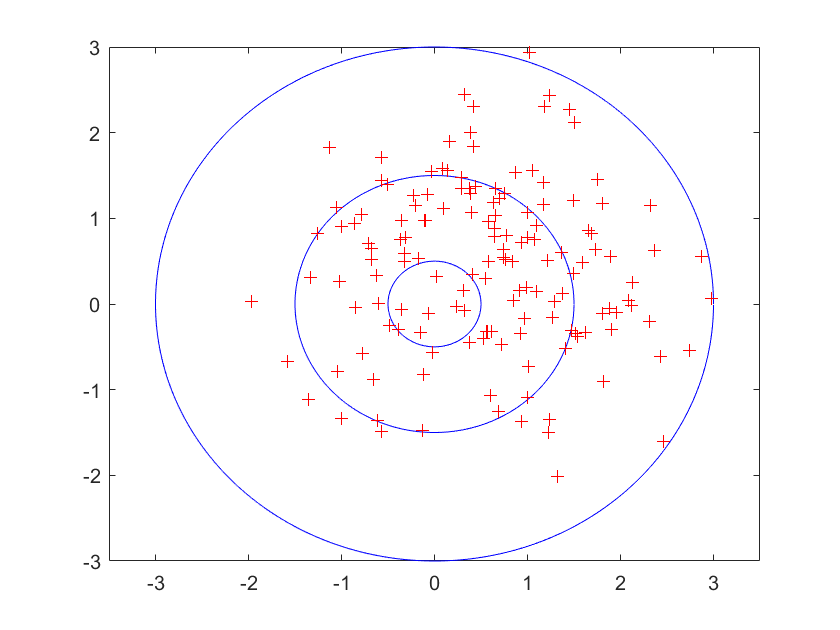
\includegraphics[width=0.75\textwidth]{bullseye.png}
\end{figure}
\end{frame}

%%%%%%%%%%%%%%%%%%%%%%%%%%%%%
\begin{frame}{Multivariate Normal}

\begin{figure}
	\centering
	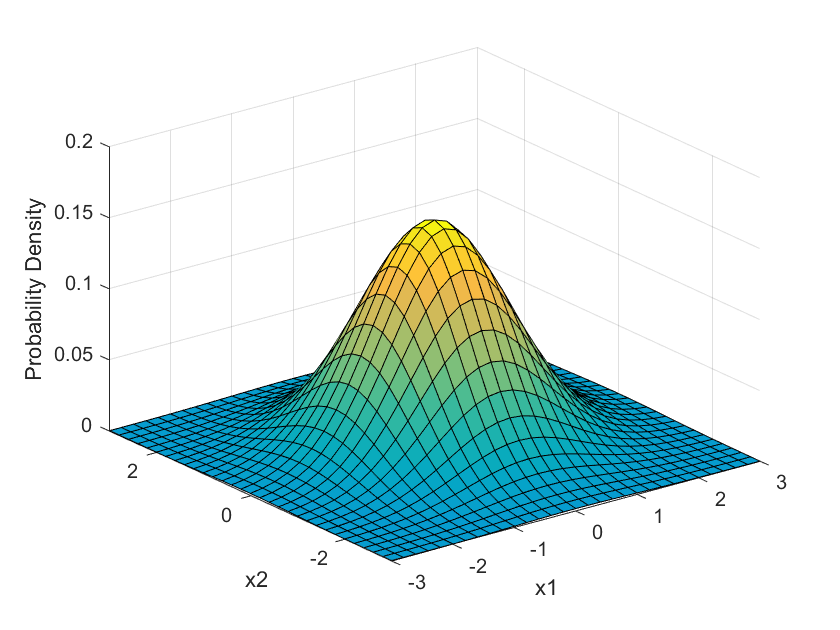
\includegraphics[width=0.5\textwidth]{MVN.png}
\end{figure}


A random vector which is multivariate normally distributed  with mean $\mathbf{\mu}$ and covariance matrix $\mathbf{\Sigma}$, written $\x \sim N(\mathbf{\mu}, \mathbf{\Sigma})$, has the following density function\bigskip

\[f(\x) = \frac{1}{\sqrt{(2\pi)^k |\mathbf{\Sigma}|}} \exp \left ( -\frac{1}{2}(\x - \mathbf{\mu})^\prime \mathbf{\Sigma}^{-1}(\x - \mathbf{\mu})  \right )\]

\end{frame}

%%%%%%%%%%%%%%%%%%%%%%%%%%%%%
\begin{frame}{Multivariate Normal}
\begin{block}{Proposition}
Let $[X_{1}, \dots, X_{n}]^{\prime} \sim N(\mathbf{0}, \mathbf{\Sigma})$. If $X_{i}$ and $X_{j}$ are uncorrelated $i \not = j$, then $X_{i}$ and $X_{j}$ are independent.
\end{block}

\vfill \vfill
\end{frame}
%%%%%%%%%%%%%%%%%%%%%%%%%%%%%
\begin{frame}{Multivariate Normal}

\begin{block}{Proposition}
Let $\x \sim N(\mathbf{\mu}, \mathbf{\Sigma})$. Then for some non-zero matrix $A$ (or vector) we have
\[ \mathbf{A}\x \sim N(\mathbf{A}\mathbf{\mu}, \mathbf{A} \mathbf{\Sigma} \mathbf{A}^\prime)\]
\end{block}

\vfill
\begin{exercise}
Suppose $X\sim N(0,1)$ and $Y \sim N(0,1)$ such that $\mathrm{Cov}(X,Y) = 0.5$. What distribution does $X - Y$ have? Confirm this with a Monte Carlo experiment.
\end{exercise}
\end{frame}

%%%%%%%%%%%%%%%%%%%%%%%%%%%%%
\begin{frame}{Distribution of Quadratic Forms}

\begin{block}{Proposition}
Let $\x \sim N(\mathbf{0}, \mathbf{I})$ be a $k \times 1$ MVN random vector. 
\[ \x^\prime \x \sim \chi^2(k)\]
\end{block}


You can think about this as a quadratic form in the identity matrix: $\x^\prime \mathbf{I} \x$.
\vfill\vfill

\end{frame}

%%%%%%%%%%%%%%%%%%%%%%%%%%%%%
\begin{frame}{Distribution of Quadratic Forms}

\begin{theorem}
Let $\x \sim N(\mathbf{0}, \sigma^2\mathbf{I})$ and let $M$ be a symmetric idempotent matrix of rank $m$. Then
\[\frac{\x^\prime M \x}{\sigma^2} \sim \chi^2(m)\]
\end{theorem}
\begin{exercise}
Proof:
\end{exercise}
\vfill\vfill
\end{frame}

%%%%%%%%%%%%%%%%%%%%%%%%%%%%%
\begin{frame}{Inequalities}

\begin{theorem}[Markov's Inequality]
If X is a random variable that takes only nonnegative values, then for any value $a > 0$
\[\P(X \geq a) \leq \frac{\E[X]}{a}\]
\end{theorem}

\textit{Proof:}
\begin{align*}
\E[X] &= \int_{0}^{\infty} x f(x)\mathrm{d}x\\
& = \int_{0}^{a}xf(x)\mathrm{d}x + \int_{a}^{\infty}xf(x)\mathrm{d}x\\
&\geq \int_{a}^{\infty}xf(x)\mathrm{d}x\\
&\geq \int_{a}^{\infty}af(x)\mathrm{d}x\\
&= a \P(X \geq a)
\end{align*}

\end{frame}

%%%%%%%%%%%%%%%%%%%%%%%%%%%%%
\begin{frame}{Inequalities}

\begin{theorem}[Chebyshev's Inequality]
If X is a random variable with mean $\mu$ and variance $\sigma^{2}$, then for any $\epsilon > 0$
\[\P(|X - \mu| > \epsilon) \leq \frac{\sigma^{2}}{\epsilon^{2}}\]
\end{theorem}
\textit{Proof:}
Since $(X - \mu)^{2}$ is a nonnegative random variable, we can apply Markov's inequality to obtain
\[\P\left( (X - \mu)^{2} \geq \epsilon^{2}\right) \leq \frac{\E[(X - \mu)^{2}]}{\epsilon^{2}}\]

But since $(X - \mu)^{2} \geq \epsilon^{2}$ iff $|X - \mu| > \epsilon$, 

\[\P(|X-\mu|\geq\epsilon) \leq \frac{\sigma^{2}}{\epsilon^{2}}\]

\end{frame}
%%%%%%%%%%%%%%%%%%%%%%%%%%%%%
\begin{frame}{Inequalities}

\begin{theorem}[Jensen's Inequality]
Let $X$ be a random variable and $f(\cdot)$ be a convex function. Then
\[f(\E[X]) \leq \E[f(X)]\]
\end{theorem}

\vfill\vfill
\end{frame}
%%%%%%%%%%%%%%%%%%%%%%%%%%%%%
\begin{frame}{Learning Outcomes}
\bc{You should be able to:}
\begin{itemize}
	\item Calculate probabilities using the appropriate laws.
	\item Calculate expectations, variances, and covariances.
	\item Manipulate moment generating functions.
	\item Apply laws relating to random vectors.
	\item Apply inequalities where appropriate.
\end{itemize}
\end{frame}
\end{document}